% 本章节介绍Qemu的原理
\section{Qemu \& KVM 基本原理}
\subsection{虚拟化}
根据维基百科关于虚拟化的定义是:“In computing,virtualization refers to the act of creating a virtual(rather than actual)version of something,including virtual computer hardware platforms,storage devices,and computer network resources。”(在计算机领域,虚拟化指创建某事物的虚拟(而非实际)版本,包括虚拟的计算机硬件平台、存储设备,以及计算机网络资源)可见,虚拟化是一种资源管理技术,它将计算机的各种实体资源(CPU、内存、存储、网络等)予以抽象和转化出来,并提供分割、重新组合,以达到最大化利用物。

\subsubsection{软件虚拟化}
就是Qemu来实现VMM层,通过纯软件的环境来模拟执行客户机里的指令。Qemu是软件层面实现二进制翻译(二进制翻译(binary translation)是指将使用某套指令集的二进制代码转换成基于另一套指令集的。)出目标平台代码交给客户机,客户机的每一条目标平台指令都会被QEMU截取,并翻译成宿主机平台的指令,然后交给实际的物理平台执行。

\subsubsection{硬件虚拟化}
这里以x86结构为例,Intel在2005年就加入硬件虚拟化的支持——Intel VT。简单来说就是计算机硬件本身有让客户机指令独立执行的能力,不完全需要VMM截获重定向。

其实客户机在Linux上就是一个进程,客户机访问自己的物理内存,实际上就是Linux内核管理的虚拟内存,以前是使用软件实现客户机虚拟地址(GVA)到客户机物理地址(GPA)再到宿主机虚拟地址(HVA)最后到宿主机物理地址(HPA)的四步转换,这个机制也称为“影子页表”,但是执行代价很大,后来这种靠软件实现的方式被硬件逻辑取代,这就是Intel的EPT技术(或者AMD的NPT技术),靠硬件自动算出GPA到HPA的过程。

\subsection{硬件虚拟化介绍}

\subsubsection{CPU虚拟化}
Intel在处理器级别提供了对虚拟化技术的支持,被称为VMX(virtual-machine
extensions)。有两种VMX操作模式:VMX根操作(root operation)与VMX非根操作
(non-root operation)。作为虚拟机监控器中的KVM就是运行在根操作模式下,而虚拟机
客户机的整个软件栈(包括操作系统和应用程序)则运行在非根操作模式下。进入VMX
非根操作模式被称为“VM Entry”;从非根操作模式退出,被称为“VM Exit”。

VMX的根操作模式与非VMX模式下最初的处理器执行模式基本一样,只是它现在支
持了新的VMX相关的指令集以及一些对相关控制寄存器的操作。VMX的非根操作模式是
一个相对受限的执行环境,为了适应虚拟化而专门做了一定的修改;在客户机中执行的一
些特殊的敏感指令或者一些异常会触发“VM Exit”退到虚拟机监控器中,从而运行在VMX
根模式。正是这样的限制,让虚拟机监控器保持了对处理器资源的控制。

一个虚拟机监控器软件的最基础的运行生命周期及其与客户机的交互如图 \ref{fig:VMM_Guest} 所示。
\begin{figure}[htbp]
    \centering
    \def\svgwidth{\columnwidth}
    \import{./figs/RISC-V/KVM/VMM_Guest/}{VMM_Guest.pdf_tex}
    \caption{VMM与Guest之间的交互}
    \label{fig:VMM_Guest}
\end{figure}
软件通过执行VMXON指令进入VMX操作模式下;在VMX模式下通过VMLAUNCH和VMRESUME指令进入客户机执行模式,即VMX非根模式;当在非根模式下触发VM Exit时,处理器执行控制权再次回到宿主机的虚拟机监控器上;最后虚拟机监控可以执行VMXOFF指令退出VMX执行模式。

逻辑处理器在根模式和非根模式之间的切换通过一个叫作VMCS(virtual-machinecontrol data structure)的数据结构来控制;而VMCS的访问是通过VMCS指针来操作的。VMCS指针是一个指向VMCS结构的64位的地址,使用VMPTRST和VMPTRLD指令对VMCS指针进行读写,使用MREAD、VMWRITE和VMCLEAR等指令对VMCS实现配置。

对于一个逻辑处理器,它可以维护多个VMCS数据结构,但是在任何时刻只有一个VMCS在当前真正生效。多个VMCS之间也是可以相互切换的,VMPTRLD指令就让某个VMCS在当前生效,而其他VMCS就自然成为不是当前生效的。一个虚拟机监控器会为一个虚拟客户机上的每一个逻辑处理器维护一个VMCS数据结构。

\subsubsection{内存虚拟化}
内存虚拟化的目的是给虚拟客户机操作系统提供一个从0地址开始的连续物理内存空间,同时在多个客户机之间实现隔离和调度。

在虚拟环境下内存地址如图 \ref{fig:Virtual2Physical_Address} 所示。
\begin{figure}[htbp]
    \centering
    \def\svgscale{0.5}
    \import{./figs/RISC-V/KVM/Virtual2Physical_Address/}{Virtual2Physical_Address.pdf_tex}
    \caption{虚拟化环境下的内存地址}
    \label{fig:Virtual2Physical_Address}
\end{figure}

内存虚拟化就是要将客户机虚拟地址(GVA)转化为最终能够访问的宿主机上的物理地址(HPA)。对于客户机操作系统而言,它不感知内存虚拟化的存在,在程序访问客户机中虚拟地址时,通过CR3寄存器可以将其转化为物理地址,但是在虚拟化环境中这个物理地址只是客户机的物理地址,还不是真实内存硬件上的物理地址。所以,虚拟机监控器就需要维护从客户机虚拟地址到宿主机物理地址之间的一个映射关系,在没有硬件提供的内存虚拟化之前,这个维护映射关系的页表叫作影子页表(Shadow Page Table)。内存的访问和更新通常是非常频繁的,要维护影子页表中对应关系会非常复杂,开销也较大。同时需要为每一个客户机都维护一份影子页表,当客户机数量较多时,其影子页表占用的内存较大也会是一个问题。

Intel CPU在硬件设计上就引入了EPT(Extended Page Tables,扩展页表),从而将客户机虚拟地址到宿主机物理地址的转换通过硬件来实现。当然,这个转换是通过两个步骤来实现的,如图2-3所示。首先,通过客户机CR3寄存器将客户机虚拟地址转化为客户机物理地址,然后通过查询EPT来实现客户机物理地址到宿主机物理地址的转化。EPT的控制权在虚拟机监控器中,只有当CPU工作在非根模式时才参与内存地址的转换。使用EPT后,客户机在读写CR3和执行INVLPG指令时不会导致VM Exit,而且客户页表结构自身导致的页故障也不会导致VM Exit。所以通过引入硬件上EPT的支持,简化了内存虚拟化的实现复杂度,同时也提高了内存地址转换的效率。


\subsubsection{I/O虚拟化}
在虚拟化的架构下,虚拟机监控器必须支持来自客户机的I/O请求。通常情况下有以下4种I/O虚拟化方式。
1)设备模拟:在虚拟机监控器中模拟一个传统的I/O设备的特性,比如在QEMU中模拟一个Intel的千兆网卡或者一个IDE硬盘驱动器,在客户机中就暴露为对应的硬件设备。客户机中的I/O请求都由虚拟机监控器捕获并模拟执行后返回给客户机。

2)前后端驱动接口:在虚拟机监控器与客户机之间定义一种全新的适合于虚拟化环境的交互接口,比如常见的virtio协议就是在客户机中暴露为virtio-net、virtio-blk等网络和磁盘设备,在QEMU中实现相应的virtio后端驱动。

3)设备直接分配:将一个物理设备,如一个网卡或硬盘驱动器直接分配给客户机使用,这种情况下I/O请求的链路中很少需要或基本不需要虚拟机监控器的参与,所以性能很好。

4)设备共享分配:其实是设备直接分配方式的一个扩展。在这种模式下,一个(具有特定特性的)物理设备可以支持多个虚拟机功能接口,可以将虚拟功能接口独立地分配给不同的客户机使用。如SR-IOV就是这种方式的一个标准协议。

表\ref{fig:I/O_virtual}展示了这4种I/O虚拟化方式的优缺点,前两种都是纯软件的实现,后两种都需要特定硬件特性的支持。

% 插入表格
\begin{table}[htbp]
     \centering
\begin{tabular}{|c|l|l|}
\hline
\multicolumn{1}{|l|}{} & \textbf{优点}                                                 & \textbf{缺点}                                                                              \\ \hline
设备模拟                   & 兼容性好,不需要额外驱动                                                & \begin{tabular}[c]{@{}l@{}}1.性能较差\\ 2.模拟设备的功能特性支持不够多\end{tabular}                        \\ \hline
前后端接口                  & 性能有所提升                                                      & \begin{tabular}[c]{@{}l@{}}1.兼容性差一些:依赖客户机总安装特定驱动\\ 2.I/O压力大时,后端驱动的CPU资源占用较高\end{tabular} \\ \hline
设备直接分配                 & 性能非常好                                                       & \begin{tabular}[c]{@{}l@{}}1.需要硬件设备的特性支持\\ 2.单个设备只能分配一个客户机\\ 3.很难支持动态迁移\end{tabular}     \\ \hline
设备共享分配                 & \begin{tabular}[c]{@{}l@{}}1.性能非常好\\ 2.单个设备可共享\end{tabular} & \begin{tabular}[c]{@{}l@{}}1.所需设备硬件的特性支持\\ 2.很难支持动态迁移\end{tabular}                       \\ \hline
\end{tabular}
\caption{常见I/O虚拟化方式的优缺点}
\label{fig:I/O_virtual}
\end{table}


\subsection{KVM \& Qemu模拟器介绍}
首先Qemu(Quick Emulator)本身并不完全是KVM的一部分,它是一套由软件模拟实现的。

而KVM(Kernel Virtual Machine)是有两部分组成,一部分是Linux内核的KVM模块,另一块是经过简化后的Qemu。它能够让Linux主机成为一个Hypervisor(虚拟机监控器)。在支持VMX(Virtual    Machine Extension)功能的x86处理器中,Linux在原有的用户模式和内核模式中新增加了客户模式,并且客户模式也拥有自己的内核模式和用户模式,虚拟机就是运行在客户模式中。三层结构如   图\ref{fig:kvm}所示。

\begin{figure}[htbp]
    \centering
    \def\svgscale{0.5}
    \import{./figs/RISC-V/KVM/KVM_3model/}{kvm_3model.pdf_tex}
    \caption{KVM三种模式的层次关系}
    \label{fig:kvm}
\end{figure}    
%『h』当前位置。将图形放置在正文文本中给出该图形环境的地方。如果本页所剩的页面不够,这一参数将不起作用。
%『t』顶部。将图形放置在页面的顶部。
%『b』底部。将图形放置在页面的底部。
%『p』浮动页。将图形放置在一只允许有浮动对象的页面上。

KVM就是在硬件辅助虚拟化技术之上构建起来的虚拟机监控器。

当然,并非要所有这些硬件虚拟化都支持才能运行KVM虚拟化,KVM对硬件最低的依赖是CPU的硬件虚拟化支持。

\subsubsection{KVM内核模块}
KVM模块是KVM虚拟化的核心模块,它在内核中由两部分组成:一个是处理器架构无关的部分,用lsmod命令中可以看到,如图 \ref{fig:lsmod_kvm} 所示,叫作kvm模块;另一个是处理器架构相关的部分,在Intel平台上就是$kvm\_intel$这个内核模块。KVM的主要功能是初始化CPU硬件,打开虚拟化模式,然后将虚拟客户机运行在虚拟机模式下,并对虚拟客户机的运行提供一定的支持。

\begin{figure}[htbp]
  \centering %居中显示
  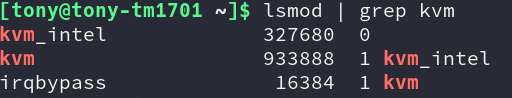
\includegraphics[width=0.9 \textwidth]{figs/RISC-V/KVM/lsmod_kvm.png}
  \caption{lsmod}
  \label{fig:lsmod_kvm} %设置图形引用名称
\end{figure}

以KVM在Intel公司的CPU上运行为例,在被内核加载的时候,KVM模块会先初始化内部的数据结构;做好准备之后,KVM模块检测系统当前的CPU,然后打开CPU控制寄存器CR4中的虚拟化模式开关,并通过执行VMXON指令将宿主操作系统(包括KVM模块本身)置于CPU执行模式的虚拟化模式中的根模式;最后,KVM模块创建特殊设备文件/dev/kvm并等待来自用户空间的命令。接下来,虚拟机的创建和运行将是一个用户空间的应用程序(QEMU)和KVM模块相互配合的过程。

/dev/kvm这个设备可以被当作一个标准的字符设备,KVM模块与用户空间QEMU的通信接口主要是一系列针对这个特殊设备文件的loctl调用。当然,每个虚拟客户机针对/dev/kvm文件的最重要的loctl调用就是“创建虚拟机”。在这里,“创建虚拟机”可以理解成KVM为了某个特定的虚拟客户机(用户空间程序创建并初始化)创建对应的内核数据结构。同时,KVM还会返回一个文件句柄来代表所创建的虚拟机。针对该文件句柄的loctl调用可以对虚拟机做相应的管理,比如创建用户空间虚拟地址和客户机物理地址及真实内存物理地址的映射关系,再比如创建多个可供运行的虚拟处理器(vCPU)。同样,KVM模块会为每一个创建出来的虚拟处理器生成对应的文件句柄,对虚拟处理器相应的文件句柄进行相应的loctl调用,就可以对虚拟处理器进行管理。

针对虚拟处理器的最重要的loctl调用就是“执行虚拟处理器”。通过它,用户空间准备好的虚拟机在KVM模块的支持下,被置于虚拟化模式中的非根模式下,开始执行二进制指令。在非根模式下,所有敏感的二进制指令都会被处理器捕捉到,处理器在保存现场之后自动切换到根模式,由KVM决定如何进一步处理(要么由KVM模块直接处理,要么返回用户空间交由用户空间程序处理)。

除了处理器的虚拟化,内存虚拟化也是由KVM模块实现的,包括前面提到的使用硬件提供的EPT特性,通过两级转换实现客户机虚拟地址到宿主机物理地址之间的转换。

处理器对设备的访问主要是通过I/O指令和MMIO,其中I/O指令会被处理器直接截获,MMIO会通过配置内存虚拟化来捕捉。但是,外设的模拟一般不由KVM模块负责。一般来说,只有对性能要求比较高的虚拟设备才会由KVM内核模块来直接负责,比如虚拟中断控制器和虚拟时钟,这样可以大量减少处理器模式切换的开销。而大部分的输入输出设备交给下一节将要介绍的用户态程序QEMU来负责。

\subsubsection{QEMU用户态设备模拟}
QEMU原本就是一个著名的开源虚拟机软件项目,而不是KVM虚拟化软件的一部分。与KVM不同,QEMU最初实现的虚拟机是一个纯软件的实现,通过二进制翻译来实现虚拟化客户机中的CPU指令模拟,所以性能比较低。但是,其优点是跨平台,QEMU支持在Linux、Windows、FreeBSD、Solaris、MacOS等多种操作系统上运行,能支持在QEMU本身编译运行的平台上就实现虚拟机的功能,甚至可以支持客户机与宿主机并不是同一个架构(比如在x86平台上运行ARM客户机)。作为一个存在已久的虚拟机监控器软件,QEMU的代码中有完整的虚拟机实现,包括处理器虚拟化、内存虚拟化,以及KVM也会用到的虚拟设备模拟(比如网卡、显卡、存储控制器和硬盘等)。

除了二进制翻译的方式,QEMU也能与基于硬件虚拟化的Xen、KVM结合,为它们提供客户机的设备模拟。通过与KVM的密切结合,让虚拟化的性能提升得非常高,在真实的企业级虚拟化场景中发挥重要作用,所以我们通常提及KVM虚拟化时就会说“QEMU/KVM”这样的软件栈。

最早期的KVM开发者们为了简化软件架构和代码重用,根据KVM特性在QEMU的基础上进行了修改(当然这部分修改已经合并回QEMU的主干代码,故现在的QEMU已原生支持KVM虚拟化特性)。从图2-8可以看出,每一个虚拟客户机在宿主机中就体现为一个QEMU进程,而客户机的每一个虚拟CPU就是一个QEMU线程。虚拟机运行期间,QEMU会通过KVM模块提供的系统调用进入内核,由KVM模块负责将虚拟机置于处理器的特殊模式下运行。遇到虚拟机进行I/O操作时,KVM模块会从上次的系统调用出口处返回QEMU,由QEMU来负责解析和模拟这些设备。

从QEMU角度来看,也可以说QEMU使用了KVM模块的虚拟化功能,为自己的虚拟机提供硬件虚拟化的加速,从而极大地提高了虚拟机的性能。除此之外,虚拟机的配置和创建,虚拟机运行依赖的虚拟设备,虚拟机运行时的用户操作环境和交互,以及一些针对虚拟机的特殊技术(如:动态迁移),都是由QEMU自己实现的。

QEMU除了提供完全模拟的设备(如:e1000网卡、IDE磁盘等)以外,还支持virtio协议的设备模拟。virtio是一个沟通客户机前端设备与宿主机上设备后端模拟的比较高性能的协议,在前端客户机中需要安装相应的virtio-blk、virtio-scsi、virtio-net等驱动,而QEMU就实现了virtio的虚拟化后端。QEMU还提供了叫作virtio-blk-data-plane的一种高性能的块设备I/O方式,它最初在QEMU 1.4版本中被引入。virtio-blk-data-plane与传统virtio-blk相比,它为每个块设备单独分配一个线程用于I/O处理,data-plane线程不需要与原QEMU执行线程同步和竞争锁,而且它使用ioeventfd/irqfd机制,同时利用宿主机Linux上的AIO(异步I/O)来处理客户机的I/O请求,使得块设备I/O效率进一步提高。

总之,QEMU既是一个功能完整的虚拟机监控器,也在QEMU/KVM的软件栈中承担设备模拟的工作。


\subsection{KVM上层管理工具}

\subsubsection{libvirt}
libvirt是使用最广泛的对KVM虚拟化进行管理的工具和应用程序接口,已经是事实上的虚拟化接口标准,本节后部分介绍的其他工具都是基于libvirt的API来实现的。作为通用的虚拟化API,libvirt不但能管理KVM,还能管理VMware、Hyper-V、Xen、VirtualBox等其他虚拟化方案。

\subsubsection{virsh}
virsh是一个常用的管理KVM虚拟化的命令行工具,对于系统管理员在单个宿主机上进行运维操作,virsh命令行可能是最佳选择。virsh是用C语言编写的一个使用libvirt API的虚拟化管理工具,其源代码也是在libvirt这个开源项目中的。

\subsubsection{virt-manager}
virt-manager是专门针对虚拟机的图形化管理软件,底层与虚拟化交互的部分仍然是调用libvirt API来操作的。virt-manager除了提供虚拟机生命周期(包括:创建、启动、停止、打快照、动态迁移等)管理的基本功能,还提供性能和资源使用率的监控,同时内置了VNC和SPICE客户端,方便图形化连接到虚拟客户机中。virt-manager在RHEL、CentOS、Fedora等操作系统上是非常流行的虚拟化管理软件,在管理的机器数量规模较小时,virt-manager是很好的选择。因其图形化操作的易用性,成为新手入门学习虚拟化操的首选管理软件。












